\documentclass[11pt]{article}

\usepackage[margin=0.65in]{geometry}
\usepackage{amsmath,amssymb}
\usepackage{array,booktabs}
\usepackage{enumitem}
\usepackage{listings}
\usepackage{xcolor}
\usepackage{tikz}
\usetikzlibrary{arrows.meta,positioning}
\usepackage{hyperref}
\usepackage{graphicx}

\setlength{\parindent}{0pt}
\setlength{\parskip}{0.5em}
\setlist[itemize]{leftmargin=1.35em}
\setlist[enumerate]{leftmargin=1.65em}

\lstdefinestyle{python}{
    language=Python,
    basicstyle=\ttfamily\small,
    columns=fullflexible,
    keepspaces=true,
    showstringspaces=false,
    frame=single,
    breaklines=true,
    tabsize=4
}

\title{Integrated Lab: Pmod ADC/DAC Loopback and the Nyquist Frequency}
\author{Prof. Jordan C. Hanson}
\date{\today}

\begin{document}
\maketitle

\section{Learning Goals}
By the end of this activity, you should be able to:
\begin{itemize}
    \item identify the role of the Pmod DAC and Pmod ADC on the PYNQ-Z1 system,
    \item send a voltage from the DAC and read the digitized voltage with the ADC,
    \item generate and sample a sine wave in Python,
    \item relate the sample spacing $\Delta t$ to the sampling frequency $f_s$, and
    \item experimentally identify what changes when the signal frequency exceeds the Nyquist frequency.
\end{itemize}

\section{Hardware Setup: PYNQ-Z1 and Pmods}

Pmods are peripheral modules that add functions to the PYNQ-Z1 board. In this activity, the Pmod DA4 converts a digital value into an analog voltage, and the Pmod AD2 converts that analog voltage back into a digital measurement.

\subsection{Lab Setup}

Figure~\ref{fig:week10setup} shows the physical arrangement used in this activity. The Pmod DA4 is connected to PMODB and the Pmod AD2 is connected to PMODA. The white jumper wire carries the analog voltage produced by the DAC to the ADC input.

\begin{figure}[h!]
    \centering
    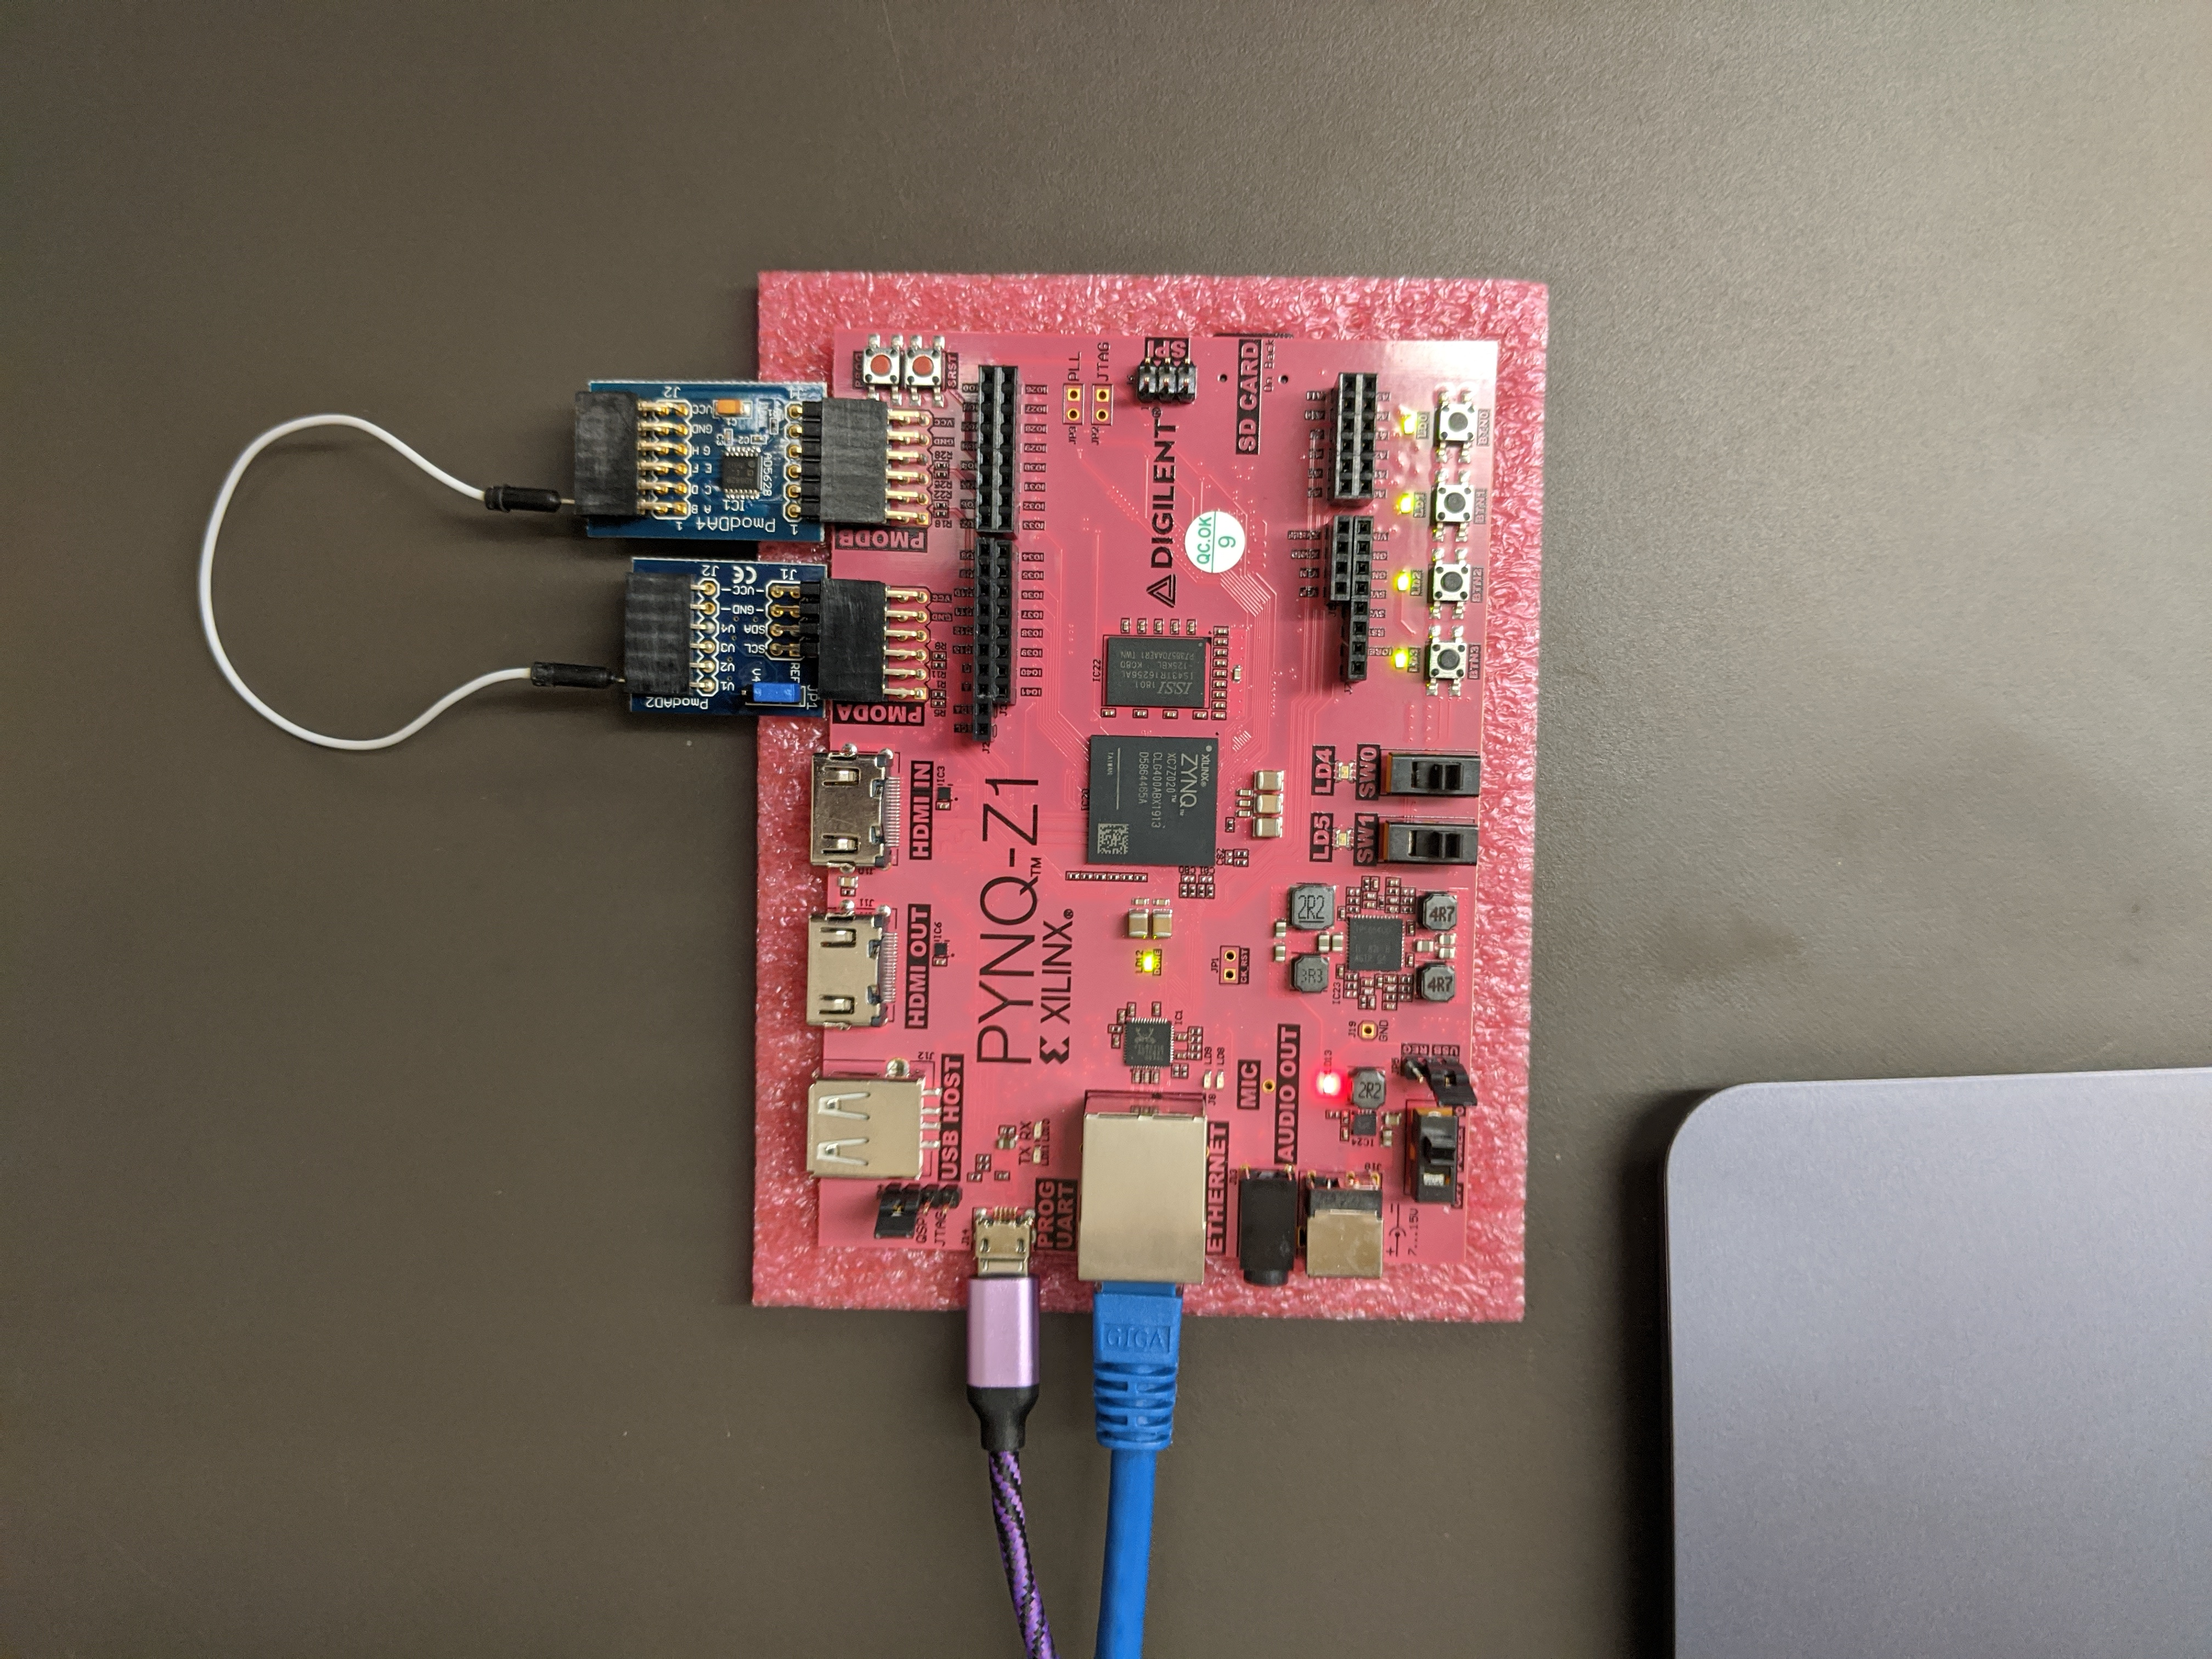
\includegraphics[width=0.5\textwidth]{week10_pmod_setup.jpg}
    \caption{Reference hardware setup from the Week 10 laboratory activity. The Pmod DA4 is connected to PMODB, the Pmod AD2 is connected to PMODA, and the white jumper wire carries the DAC analog output to the ADC analog input.}
    \label{fig:week10setup}
\end{figure}

\subsection{How to plug the Pmods into the PYNQ-Z1}

Power the board off before inserting, removing, or repositioning either Pmod. Verify the orientation before turning the board back on.

A PYNQ Pmod connector has two rows of six pins. Each row contains VCC, GND, and four digital signal pins. The VCC/GND end of the connector is the reference end for orienting both modules.

\begin{enumerate}[label=\alph*)]
    \item \textbf{Pmod DA4 on PMODB.} The DA4 uses a single row of six pins. Insert the DA4 into one complete row of \texttt{PMODB}, with the module's VCC and GND pins aligned with the VCC and GND pins on PMODB. A single-row Pmod can occupy either row of the Pmod connector; for this activity, match the orientation shown in Fig.~\ref{fig:week10setup}.

    \item \textbf{Pmod AD2 on PMODA.} The AD2 uses a 2-by-4 connector and therefore occupies \textbf{both rows} of \texttt{PMODA}. Place it at the VCC/GND end of the PMODA header; the AD2's GND and VCC pins must line up with the corresponding GND and VCC pins on the PYNQ connector. The remaining two columns at the signal-only end of PMODA remain uncovered.

    \item \textbf{ADC reference jumper.} Set your Pmod AD2 reference-selection jumper\texttt{JP1} to \texttt{REF}.
\end{enumerate}

\subsection{Connect the DAC output to the ADC input}

The Python commands used later in the activity,

\begin{lstlisting}[style=python]
dac.write(voltage)
adc.read()
\end{lstlisting}

use \textbf{DAC channel A} and \textbf{ADC channel 1} by default. Therefore, make the loopback connection as follows:

\begin{center}
\fbox{\parbox{0.82\textwidth}{
\centering
\textbf{Pmod DA4 J2 pin 1: VOUTA} $\longrightarrow$ \textbf{Pmod AD2 J2 pin 1: UIN1}
}}
\end{center}

Use one jumper wire between those two analog pins. The two Pmods already share a common ground through the PYNQ-Z1 Pmod headers, so a second ground jumper is not required for this same-board loopback setup.  Ask the instructor to verify the connection before powering the board.

\subsection{Signal Path}

The system should now be connected conceptually as follows:

\begin{center}
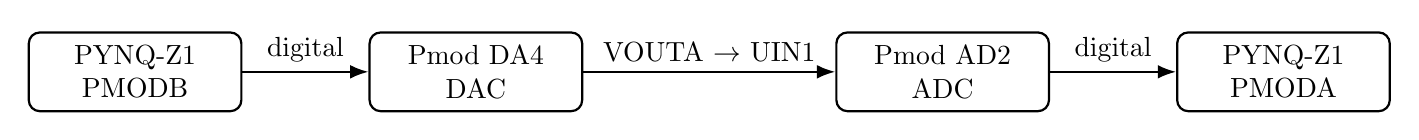
\begin{tikzpicture}[
    >=Latex,
    block/.style={draw,rectangle,rounded corners,minimum width=2.7cm,minimum height=1.0cm,align=center,thick},
    line/.style={->,thick}
]
\node[block] (pynq1) {PYNQ-Z1\\PMODB};
\node[block,right=1.6cm of pynq1] (dac) {Pmod DA4\\DAC};
\node[block,right=3.2cm of dac] (adc) {Pmod AD2\\ADC};
\node[block,right=1.6cm of adc] (pynq2) {PYNQ-Z1\\PMODA};

\draw[line] (pynq1) -- node[above]{digital} (dac);
\draw[line] (dac) -- node[above]{VOUTA $\to$ UIN1} (adc);
\draw[line] (adc) -- node[above]{digital} (pynq2);
\end{tikzpicture}
\end{center}

The AD2 used in the original activity has 12-bit resolution and is the limiting device in this loopback experiment. For this lab, treat the nominal combined ADC/DAC working range as 0--2.0 V and do not command the DAC above $2.0\,$V. This matches the range used in the Week 10 activity and leaves a small margin below ADC full scale. You may observe measurable non-linearity before full scale; if so, record the approximate voltage where the deviation becomes noticeable.

\begin{center}
\fbox{\parbox{0.82\textwidth}{
\centering
\textbf{Voltage rule for this lab:} $0 \leq V_{\mathrm{DAC}} \leq 2.0\,\mathrm{V}$.\\
Do not exceed $2.0\,$V in the loopback experiment.
}}
\end{center}

\section{Start the PYNQ/Jupyter Environment}

Open the PYNQ Jupyter environment on the laboratory computer and create a new notebook. Run the following setup cell.

\begin{lstlisting}[style=python]
%matplotlib inline
import matplotlib.pyplot as plot
from time import sleep
import numpy as np
from pynq.lib import Pmod_ADC, Pmod_DAC
from pynq.overlays.base import BaseOverlay
ol = BaseOverlay("base.bit")
dac = Pmod_DAC(ol.PMODB)
adc = Pmod_ADC(ol.PMODA)
\end{lstlisting}

\section{Verify the ADC/DAC Loopback}

Before generating a waveform, test a few constant voltages. Use the same DAC/ADC commands demonstrated in the PYNQ \texttt{getting\_started} Pmod tutorial or by your instructor.

For each requested DAC voltage, record the ADC measurement. The final two points deliberately approach the upper part of the useful range so that you can check whether the response remains linear.

\begin{center}
\renewcommand{\arraystretch}{1.3}
\begin{tabular}{ccc}
\toprule
\textbf{DAC voltage (V)} & \textbf{ADC measured voltage (V)} & \textbf{Difference (V)} \\
\midrule
0.25 & & \\
0.50 & & \\
1.00 & & \\
1.50 & & \\
1.75 & & \\
2.00 & & \\
\bottomrule
\end{tabular}
\end{center}

\begin{enumerate}[label=\alph*)]
    \item Are the measured values exactly equal to the requested values? If not, describe the size and pattern of the differences.
    \item Does the ADC/DAC response remain approximately linear all the way to $2.0\,$V? If not, estimate the voltage at which the deviation first becomes noticeable.
\end{enumerate}

\section{Generate and Sample a Sine Wave}

We will generate the analog waveform
\begin{equation}
    v(t)=A\sin(2\pi f t)+B,
\end{equation}
where $A$ is the amplitude, $B$ is the DC offset, and $f$ is the sine-wave frequency.  The sample spacing is $\Delta t$, so the nominal sampling frequency is
\begin{equation}
    f_s=\frac{1}{\Delta t}.
\end{equation}

Start with the following values:
\begin{equation*}
    f_s=10\ \mathrm{Hz},\qquad
    f=0.5\ \mathrm{Hz},\qquad
    A=0.5\ \mathrm{V},\qquad
    B=1.0\ \mathrm{V}.
\end{equation*}
These values keep the sine wave between $0.5$ and $1.5\,$V, inside the ADC range used in the original worksheet.

\begin{lstlisting}[style=python]
# Transmission loop
sampling_frequency = 10.0 #Hz
delta_t = 1.0 / sampling_frequency
t_max = 10.0 #seconds
times = np.arange(0, t_max, delta_t)
dc_offset = 1.0 #volts
amplitude = 0.5 #volts
frequency = 0.5 #Hz
samples = []
for t in times:
    voltage = amplitude*np.sin(2.0*np.pi*frequency*t) + dc_offset
    dac.write(voltage)
    sleep(delta_t)
    samples.append(adc.read())
\end{lstlisting}

Plot the measurements.

\begin{lstlisting}[style=python]
plot.plot(times, samples, '-o')
plot.title(
    "Signal frequency: " + str(frequency) +
    " Hz, sampling frequency: " + str(sampling_frequency) + " Hz"
)
plot.xlabel('Time (seconds)')
plot.ylabel('Amplitude (Volts)')
plot.grid(True)
plot.axis([0, t_max, 0, 2.0])
plot.show()
\end{lstlisting}

\textbf{Checkpoint questions}
\begin{enumerate}[label=\alph*)]
    \item What is $\Delta t$ for $f_s=10\,$Hz?
    \item How many samples are taken during one period of a $0.5\,$Hz sine wave?
    \item Does the sampled waveform resemble the expected sine wave? Describe any differences.
\end{enumerate}

\section{Explore the Nyquist Frequency}

For a sampling frequency $f_s$, the Nyquist frequency is $f_N=f_s/2$.  Keep the nominal sampling frequency fixed at $f_s=10\ \mathrm{Hz}$.  Therefore, $f_N=\underline{\hspace{2cm}}\ \mathrm{Hz}$.  Change only the sine-wave frequency and repeat the transmission/measurement plot for the cases below.

\begin{center}
\renewcommand{\arraystretch}{1.35}
\begin{tabular}{c c c p{5.3cm}}
\toprule
\textbf{$f$ (Hz)} & \textbf{$f/f_s$} & \textbf{Samples/cycle} & \textbf{What do you observe?} \\
\midrule
1.0 & & & \\
2.5 & & & \\
4.0 & & & \\
5.0 & & & \\
6.0 & & & \\
8.0 & & & \\
\bottomrule
\end{tabular}
\end{center}

\begin{enumerate}[label=\alph*)]
    \item Which plots clearly reproduce the original sine-wave shape?
    \item What is special about the case $f=f_s/2$?
    \item What happens when $f>f_s/2$?
    \item For the cases above the Nyquist frequency, does the sampled data appear to oscillate at a frequency different from the frequency you programmed? Describe what you see.
    \item Based on your measurements, write a one- or two-sentence experimental statement of the Nyquist-Shannon sampling condition.
\end{enumerate}

\section{Change the Sampling Frequency}

Now choose a fixed sine-wave frequency of $f=2.0\ \mathrm{Hz}$.  Repeat the experiment.

\begin{center}
\renewcommand{\arraystretch}{1.35}
\begin{tabular}{c c c p{5.0cm}}
\toprule
\textbf{$f_s$ (Hz)} & \textbf{$f_N$ (Hz)} & \textbf{Samples/cycle} & \textbf{Observed waveform} \\
\midrule
20 & & & \\
10 & & & \\
6 & & & \\
4 & & & \\
3 & & & \\
\bottomrule
\end{tabular}
\end{center}

\begin{enumerate}[label=\alph*)]
    \item At what sampling frequency does the waveform first become difficult to recognize?
    \item Compare the $f_s=4\,$Hz result to the $f_s=3\,$Hz result. Why are they qualitatively different?
    \item If you wanted a visually smooth reconstruction rather than merely satisfying the theoretical limit, would you choose $f_s=2f$, or a substantially larger sampling frequency? Explain from your plots.
\end{enumerate}

\section{Reflection}

Answer each question briefly. (a) In this experiment, what physical quantity does the DAC produce? (b) What physical quantity does the ADC measure? (c) What role does \texttt{delta\_t} play in the experiment? (d) What is the relationship between \texttt{delta\_t}, $f_s$, and the Nyquist frequency? (e) Why can two different continuous-time sine-wave frequencies produce sampled data that look deceptively similar when the Nyquist condition is violated?

\end{document}
